\begin{frame}[fragile]
  \begin{verbatim}
checker = InteractiveInvariantConfluenceChecker()
x = checker.int_max('x', 0) # An int, x, merged by max.
y = checker.int_max('y', 0) # An int, y, merged by max.
checker.add_transaction('inc_x', [x.assign(x + 1)])
checker.add_transaction('dec_y', [y.assign(y - 1)])
checker.add_invariant(x * y <= 0)
checker.check()\end{verbatim}

  \note{%
    Finally, I'll give a teaser of our evaluation. We implemented our decision
    procedure in Python and leveraged the Z3 decision procedure. You can
    specify objects, transactions, and invariants with code that looks like
    this. \\[12pt]

    This code specifies the running example that we've been looking at
    throughout the talk. $x$ is an integer merged by max that is initially 0.
    $y$ is an integer merged by max that is initially 0. We have a transaction
    incx that increments x and a function decy that decrements y. And, our
    invariant is that the product of $x$ and $y$ is less than or equal to zero.
  }
\end{frame}

\begin{frame}
  \begin{itemize}
    \item Foreign keys
    \item Auction application
    \item Escrow transactions
    \item TPC-C
  \end{itemize}

  \pause
  All run in less than a second and are implemented in less than 75 lines of
  specification.

  \note{%
    In our paper, we specified a bunch of examples including things involving
    foreign keys, an auction application, something involving escrow
    transactions, and TPC-C.  All the examples verify with a runtime of less
    then a second and every one is implemented in fewer than 75 lines of
    specification.
  }
\end{frame}

\begin{frame}
  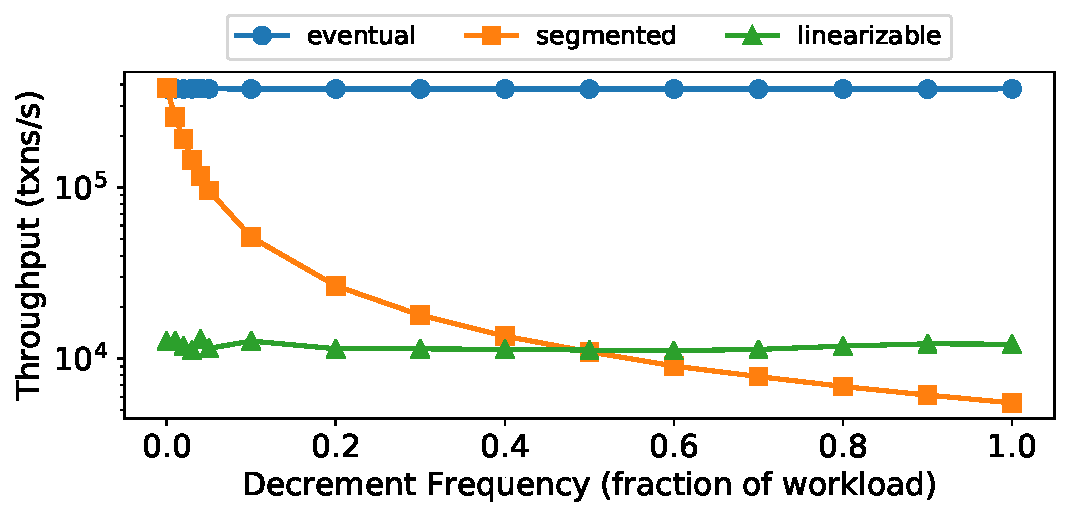
\includegraphics[width=\textwidth]{assets/throughput_vs_fraction_16.pdf}

  \note{%
    We have some graphs showing that no coordination vastly outperforms
    replicating with strong consistency, and how segmented invariant confluence
    allows a smooth tradeoff between the two. Fully invariant confluent objects
    don't require any coordination, partly invariant confluent objects require
    some coordination, and not at all invariant confluent objects require a lot
    of coordination.
  }
\end{frame}

\begin{frame}
  \begin{center}
    \Huge
    Come to our poster tomorrow night!
  \end{center}

  \note{%
    I've jumped over a ton of details in the paper, and some things I didn't
    even mention at all. If you're curious about anything, I encourage you to
    come to our poster tomorrow night where I'm happy to chat.
  }
\end{frame}

\begin{frame}
  \begin{center}
    \Huge
    Thank you
  \end{center}

  \note{%
    Thank you all for listening, and I'm happy to take questions.
  }
\end{frame}
